\documentclass[12pt]{article}
\usepackage{amsfonts, amssymb, amsmath, amsthm}
\usepackage[margin=1in]{geometry}
\usepackage{tikz}
\usetikzlibrary{patterns, decorations.pathreplacing}

\pagestyle{myheadings}
\markright{Explainer: Rudin 4.18 --- Thomae's Function\hfill}

\newcommand{\R}{\mathbb{R}}
\newcommand{\Q}{\mathbb{Q}}
\newcommand{\N}{\mathbb{N}}
\newcommand{\eps}{\varepsilon}

\begin{document}

\begin{center}
    \textbf{\Large Thomae's Function (The Ruler Function)}\\[0.5em]
    \large A visual guide to Rudin 4.18
\end{center}

\section{The Definition}

For $x \in \R$, define:
\[
f(x) = \begin{cases}
0 & \text{if } x \text{ is irrational,}\\[0.5em]
\displaystyle\frac{1}{n} & \text{if } x = \displaystyle\frac{m}{n} \text{ in lowest terms, } n > 0
\end{cases}
\]

\section{What Does This Function Look Like?}

\begin{center}
\begin{tikzpicture}[scale=6]
    % Axes
    \draw[thick, ->] (-0.05, 0) -- (1.1, 0) node[right] {$x$};
    \draw[thick, ->] (0, -0.05) -- (0, 0.6) node[above] {$f(x)$};

    % Tick marks on y-axis
    \foreach \n/\label in {1/1, 0.5/\frac{1}{2}, 0.333/\frac{1}{3}, 0.25/\frac{1}{4}, 0.2/\frac{1}{5}} {
        \draw (0, \n) -- (-0.01, \n) node[left] {\tiny $\label$};
    }

    % n=1: 0/1 and 1/1
    \fill[red] (0, 1*0.5) circle (0.5pt);
    \fill[red] (1, 1*0.5) circle (0.5pt);

    % n=2: 1/2
    \fill[blue] (0.5, 0.5*0.5) circle (0.5pt);

    % n=3: 1/3, 2/3
    \fill[green!50!black] (0.333, 0.333*0.5) circle (0.5pt);
    \fill[green!50!black] (0.667, 0.333*0.5) circle (0.5pt);

    % n=4: 1/4, 3/4
    \fill[orange] (0.25, 0.25*0.5) circle (0.4pt);
    \fill[orange] (0.75, 0.25*0.5) circle (0.4pt);

    % n=5: 1/5, 2/5, 3/5, 4/5
    \foreach \m in {1,2,3,4} {
        \pgfmathsetmacro{\x}{\m/5}
        \fill[purple] (\x, 0.2*0.5) circle (0.4pt);
    }

    % n=6: 1/6, 5/6
    \fill[brown] (0.167, 0.167*0.5) circle (0.35pt);
    \fill[brown] (0.833, 0.167*0.5) circle (0.35pt);

    % n=7: 1/7, 2/7, 3/7, 4/7, 5/7, 6/7
    \foreach \m in {1,2,3,4,5,6} {
        \pgfmathsetmacro{\x}{\m/7}
        \fill[gray] (\x, 0.143*0.5) circle (0.3pt);
    }

    % n=8: 1/8, 3/8, 5/8, 7/8
    \foreach \m in {1,3,5,7} {
        \pgfmathsetmacro{\x}{\m/8}
        \fill[gray] (\x, 0.125*0.5) circle (0.3pt);
    }

    % n=9: 1/9, 2/9, 4/9, 5/9, 7/9, 8/9
    \foreach \m in {1,2,4,5,7,8} {
        \pgfmathsetmacro{\x}{\m/9}
        \fill[gray!60] (\x, 0.111*0.5) circle (0.25pt);
    }

    % n=10: 1/10, 3/10, 7/10, 9/10
    \foreach \m in {1,3,7,9} {
        \pgfmathsetmacro{\x}{\m/10}
        \fill[gray!60] (\x, 0.1*0.5) circle (0.25pt);
    }

    % Irrationals on x-axis (just show the axis thickened)
    \draw[red!30, very thick] (0, 0) -- (1, 0);
    \node at (0.5, -0.07) {\small irrationals: $f = 0$};

    % Legend
    \node[text width=5cm, align=left] at (1.4, 0.35) {
        \tiny\color{red} $\bullet$ denominator 1\\
        \tiny\color{blue} $\bullet$ denominator 2\\
        \tiny\color{green!50!black} $\bullet$ denominator 3\\
        \tiny\color{orange} $\bullet$ denominator 4\\
        \tiny\color{purple} $\bullet$ denominator 5
    };
\end{tikzpicture}
\end{center}

It's called the \textbf{ruler function} because the pattern resembles markings on a ruler --- taller marks for simpler fractions!

\section{Continuous at Every Irrational}

\textbf{Claim:} At any irrational $x_0$, $f$ is continuous.

\textbf{Intuition:} $f(x_0) = 0$. We need $f(x)$ to be close to $0$ when $x$ is near $x_0$. The only points where $f$ is \emph{not} close to $0$ are rationals with small denominators --- and there are only \textbf{finitely many} of those in any bounded interval!

\begin{center}
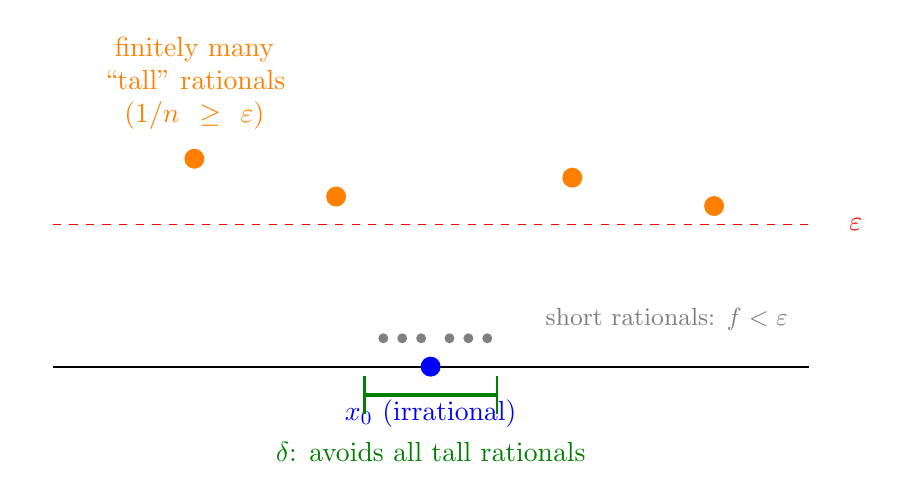
\begin{tikzpicture}[scale=1.2]
    % Number line near an irrational
    \draw[thick] (-4, 0) -- (4, 0);
    \fill[blue] (0, 0) circle (3pt);
    \node[blue] at (0, -0.5) {$x_0$ (irrational)};

    % Epsilon line
    \draw[red, dashed] (-4, 1.5) -- (4, 1.5);
    \node[red] at (4.5, 1.5) {$\eps$};

    % Rationals with big height (small denom) - finitely many!
    \fill[orange] (-2.5, 2.2) circle (3pt);
    \fill[orange] (-1, 1.8) circle (3pt);
    \fill[orange] (1.5, 2) circle (3pt);
    \fill[orange] (3, 1.7) circle (3pt);

    \node[orange, text width=4cm, align=center] at (-2.5, 3) {finitely many\\``tall'' rationals\\($1/n \geq \eps$)};

    % Delta neighborhood avoiding them
    \draw[green!50!black, very thick] (-0.7, -0.3) -- (0.7, -0.3);
    \draw[green!50!black, thick] (-0.7, -0.5) -- (-0.7, -0.1);
    \draw[green!50!black, thick] (0.7, -0.5) -- (0.7, -0.1);
    \node[green!50!black] at (0, -0.9) {$\delta$: avoids all tall rationals};

    % Small dots for rationals with big denom
    \foreach \x in {-0.5, -0.3, -0.1, 0.2, 0.4, 0.6} {
        \fill[gray] (\x, 0.3) circle (1.5pt);
    }
    \node[gray] at (2.5, 0.5) {\small short rationals: $f < \eps$};
\end{tikzpicture}
\end{center}

\subsection{The Finiteness Argument}

\begin{center}
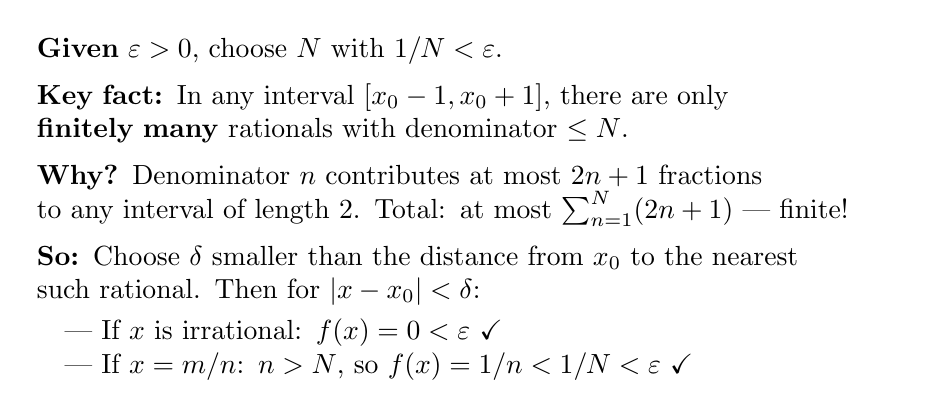
\begin{tikzpicture}[scale=1]
    \node[text width=11cm, align=left] at (0, 0) {
        \textbf{Given} $\eps > 0$, choose $N$ with $1/N < \eps$.\\[0.5em]
        \textbf{Key fact:} In any interval $[x_0 - 1, x_0 + 1]$, there are only\\
        \textbf{finitely many} rationals with denominator $\leq N$.\\[0.5em]
        \textbf{Why?} Denominator $n$ contributes at most $2n + 1$ fractions\\
        to any interval of length 2. Total: at most $\sum_{n=1}^{N}(2n+1)$ --- finite!\\[0.5em]
        \textbf{So:} Choose $\delta$ smaller than the distance from $x_0$ to the nearest\\
        such rational. Then for $|x - x_0| < \delta$:\\[0.3em]
        \quad --- If $x$ is irrational: $f(x) = 0 < \eps$ \checkmark\\
        \quad --- If $x = m/n$: $n > N$, so $f(x) = 1/n < 1/N < \eps$ \checkmark
    };
\end{tikzpicture}
\end{center}

\section{Discontinuous at Every Rational}

\textbf{Claim:} At any rational $x_0 = m/n$, $f$ has a \textbf{simple discontinuity}.

\begin{center}
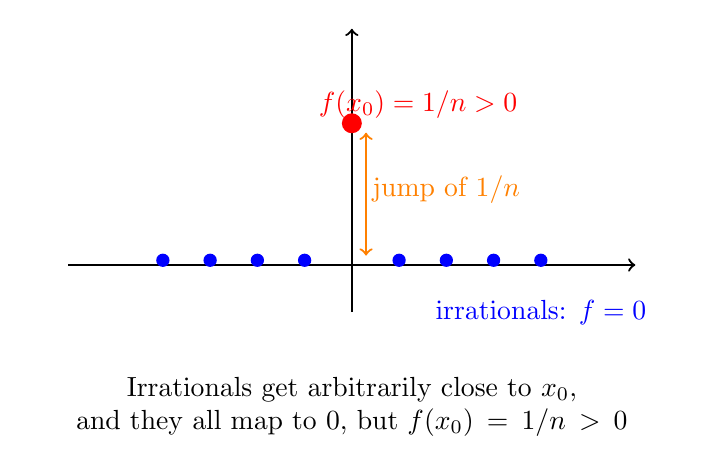
\begin{tikzpicture}[scale=1.2]
    \draw[thick, ->] (-3, 0) -- (3, 0);
    \draw[thick, ->] (0, -0.5) -- (0, 2.5);

    % x_0 = p/q
    \fill[red] (0, 1.5) circle (3pt);
    \node[red] at (0.7, 1.7) {$f(x_0) = 1/n > 0$};

    % Nearby irrationals giving 0
    \foreach \x in {-2, -1.5, -1, -0.5, 0.5, 1, 1.5, 2} {
        \fill[blue] (\x, 0.05) circle (2pt);
    }
    \node[blue] at (2, -0.5) {irrationals: $f = 0$};

    % Arrow showing the jump
    \draw[<->, orange, thick] (0.15, 0.1) -- (0.15, 1.4);
    \node[orange] at (1, 0.8) {jump of $1/n$};

    \node[text width=8cm, align=center] at (0, -1.5) {
        Irrationals get arbitrarily close to $x_0$,\\
        and they all map to $0$, but $f(x_0) = 1/n > 0$
    };
\end{tikzpicture}
\end{center}

\subsection{What ``Simple Discontinuity'' Means}

A discontinuity is \textbf{simple} if both one-sided limits exist (but may differ from $f(x_0)$).

Here: $\lim_{x \to x_0^+} f(x) = 0$ and $\lim_{x \to x_0^-} f(x) = 0$ (by the same finiteness argument --- near $x_0$, all values of $f$ are small except $f(x_0)$ itself). So the limits exist and equal $0$, but $f(x_0) = 1/n \neq 0$.

\section{The Big Picture}

\begin{center}
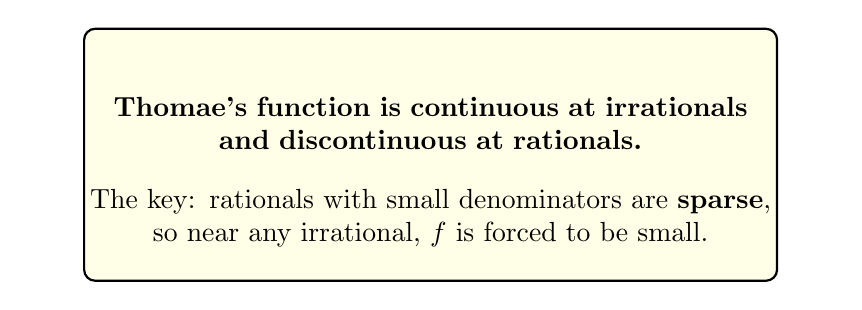
\begin{tikzpicture}[scale=0.8]
    \draw[thick, rounded corners, fill=yellow!10] (-5.5, -2) rectangle (5.5, 2);
    \node[text width=10cm, align=center] at (0, 0.5) {
        \textbf{Thomae's function is continuous at irrationals}\\
        \textbf{and discontinuous at rationals.}
    };
    \node[text width=10cm, align=center] at (0, -1) {
        The key: rationals with small denominators are \textbf{sparse},\\
        so near any irrational, $f$ is forced to be small.
    };
\end{tikzpicture}
\end{center}

\textbf{Fun fact:} No function can be continuous at every rational and discontinuous at every irrational! (The set of continuity points of any function must be a $G_\delta$ set, and the irrationals are $G_\delta$ but the rationals are not.)

\end{document}
